% --------------------------------------------------------------
% This is all preamble stuff that you don't have to worry about.
% Head down to where it says "Start here"
% --------------------------------------------------------------

\documentclass[12pt]{article}

\usepackage[margin=1in]{geometry}
\usepackage{amsmath,amsthm,amssymb}
\usepackage{graphicx} %This allows to include eps figures
\usepackage{subcaption}
\usepackage[section]{placeins}
\usepackage{layout}
\usepackage{etoolbox}
\usepackage{mathabx}
\usepackage{animate}
\usepackage{array}
% This is to include code
\usepackage{listings}
\usepackage{xcolor}
\definecolor{dkgreen}{rgb}{0,0.6,0}
\definecolor{gray}{rgb}{0.5,0.5,0.5}
\definecolor{mauve}{rgb}{0.58,0,0.82}
\lstdefinestyle{Python}{
    language        = Python,
    basicstyle      = \ttfamily,
    keywordstyle    = \color{blue},
    keywordstyle    = [2] \color{teal}, % just to check that it works
    stringstyle     = \color{green},
    commentstyle    = \color{red}\ttfamily
}

\newenvironment{conditions}
  {\par\vspace{\abovedisplayskip}\noindent\begin{tabular}{>{$}l<{$} @{${}={}$} l}}
  {\end{tabular}\par\vspace{\belowdisplayskip}}

\newcommand{\N}{\mathbb{N}}
\newcommand{\Z}{\mathbb{Z}}

\newenvironment{theorem}[2][Theorem]{\begin{trivlist}
\item[\hskip \labelsep {\bfseries #1}\hskip \labelsep {\bfseries #2.}]}{\end{trivlist}}
\newenvironment{lemma}[2][Lemma]{\begin{trivlist}
\item[\hskip \labelsep {\bfseries #1}\hskip \labelsep {\bfseries #2.}]}{\end{trivlist}}
\newenvironment{exercise}[2][Exercise]{\begin{trivlist}
\item[\hskip \labelsep {\bfseries #1}\hskip \labelsep {\bfseries #2.}]}{\end{trivlist}}
\newenvironment{reflection}[2][Reflection]{\begin{trivlist}
\item[\hskip \labelsep {\bfseries #1}\hskip \labelsep {\bfseries #2.}]}{\end{trivlist}}
\newenvironment{proposition}[2][Proposition]{\begin{trivlist}
\item[\hskip \labelsep {\bfseries #1}\hskip \labelsep {\bfseries #2.}]}{\end{trivlist}}
\newenvironment{corollary}[2][Corollary]{\begin{trivlist}
\item[\hskip \labelsep {\bfseries #1}\hskip \labelsep {\bfseries #2.}]}{\end{trivlist}}



\begin{document}

% --------------------------------------------------------------
%                         Start here
% --------------------------------------------------------------

%\renewcommand{\qedsymbol}{\filledbox}

\title{Assignment 6}%replace X with the appropriate number
\author{Nalet Meinen and Pascal Wyss\\ %replace with your name
Finite Element Analysis I
}
\maketitle

\begin{figure}[!htb]
  \centering
  \vspace*{1cm}
  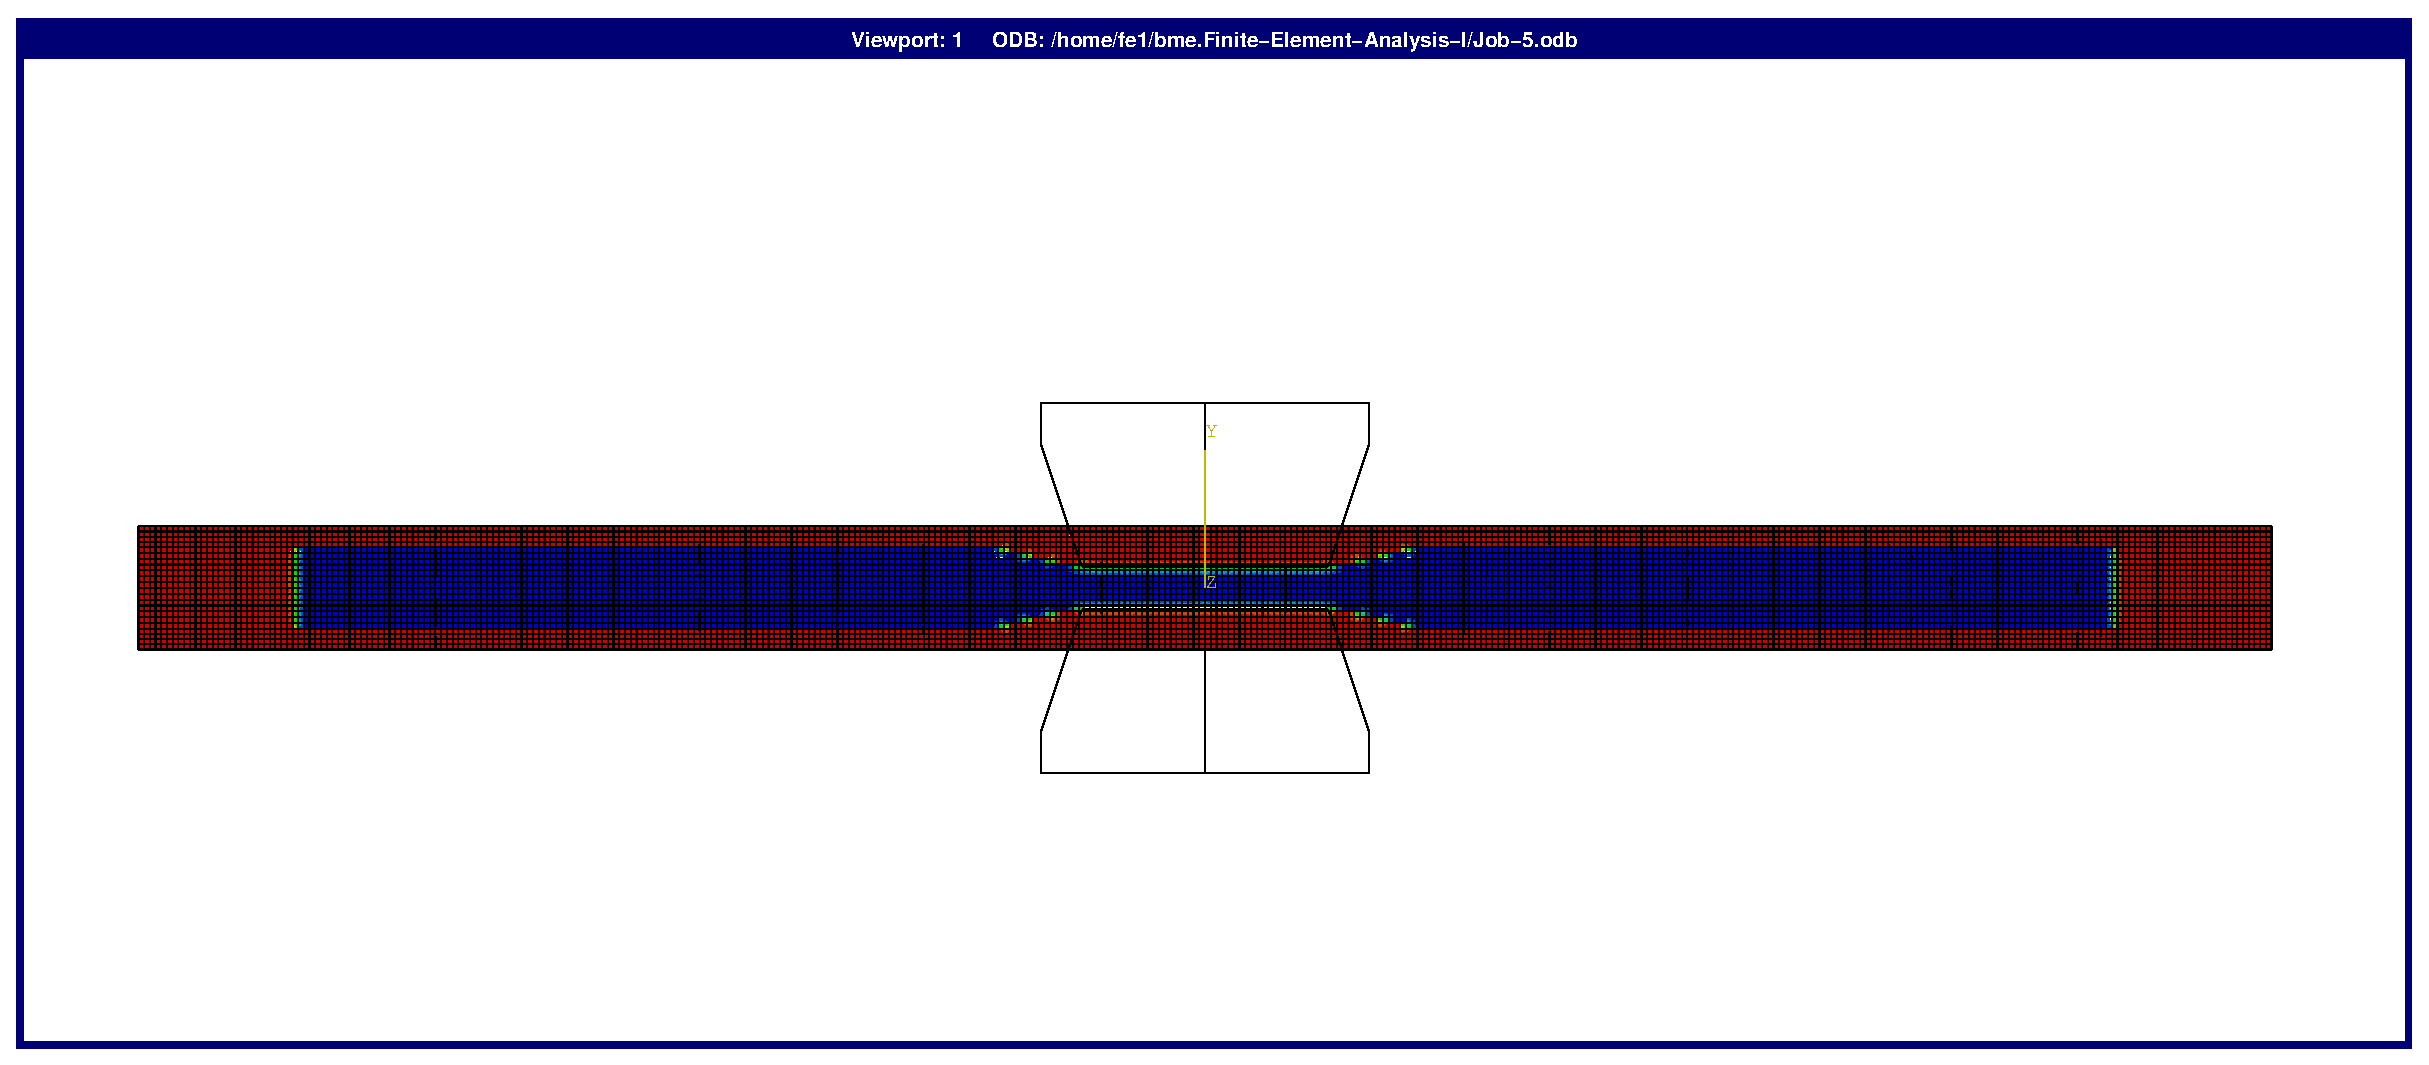
\includegraphics[trim={2cm 2cm 2cm 2cm},clip,width=1.0\linewidth]{pics/titelbild}
  \label{fig:0}
\end{figure}

\newpage

\section*{Abstract}
In this assignment we investigate the behaviour of a model cornea tissue sample 
consisitng of fibers at different angles
respective to the applied force. Those fibers represent a multi-layer biological
tissue, as usually found in the cornea, the annulus fibrosus or arterial walls (just to name a few).
The resulting foce / displacement relationship, after applying a force to the sample is our primary
matter of interest.

% \begin{figure}[!htb]
%   \centering
%   \animategraphics[autoplay,loop,width=0.8\linewidth,trim={1mm 1mm 1mm 1mm}]{4}{pics/out/ani-}{1}{62}
%   \caption{Animation of frequency on beam}
% \end{figure}

\tableofcontents
\pagebreak
\section{Introduction}

The cornea sample is modelled using abaqus. The fibers are orientated at 45 degrees respective to
the applied force. The force is applied on the top of the sample, pulling upwards.
In this simulation, a fixed deformation of factor 1.25 is performed, retrieving the corresponding 
force values.
In a second simulation, the fibers are orientated  at 30 degrees respective to the line of force,
while maintaining orthogonality between the fiber sets. We expect a less symmetric behaviour of the sample
during simulation due to the asymmetric setup.

\begin{figure}[!htb]
  \centering
  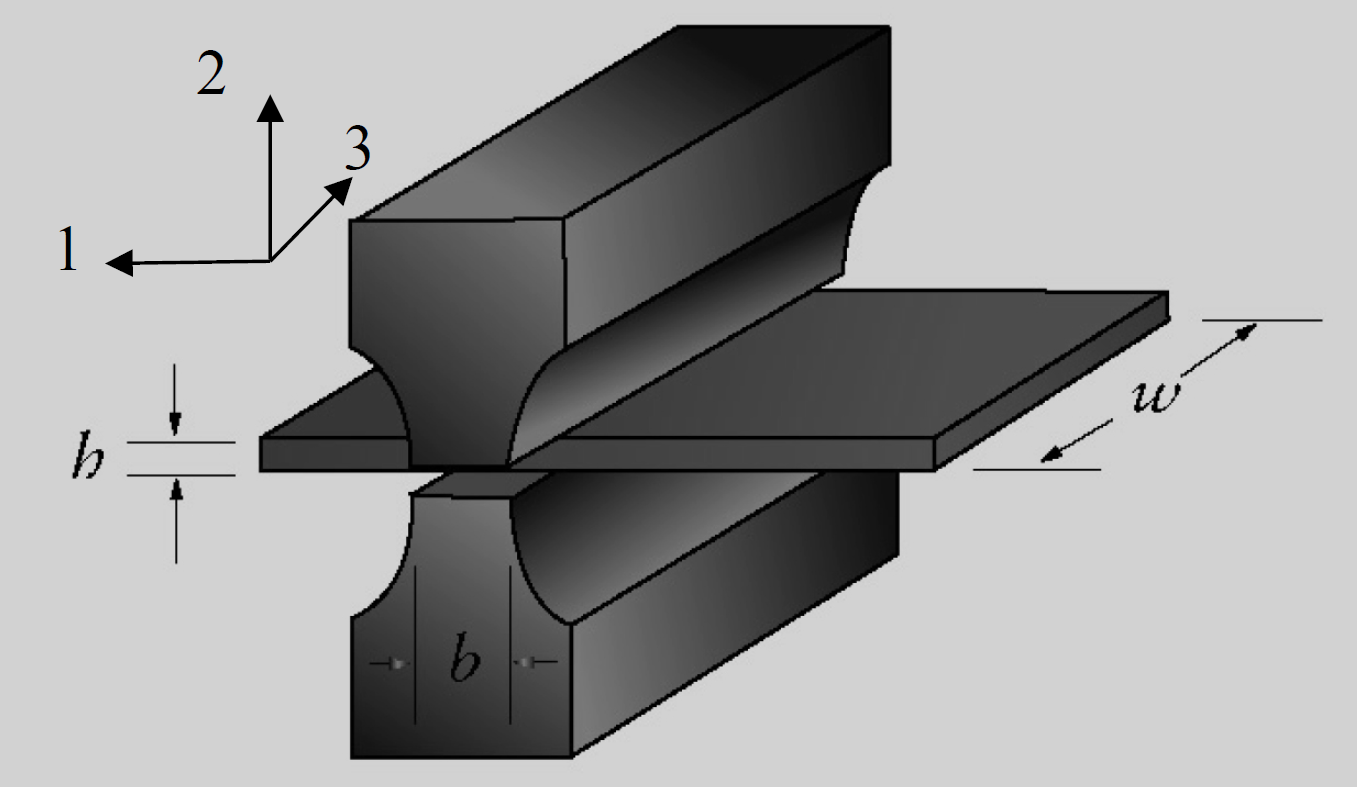
\includegraphics[width=1.0\linewidth]{pics/shematics}
  \caption{Model of the plate with Eulerian formulation}
  \label{fig:1}
\end{figure}

\noindent As shown in Figure \ref{fig:1}, the fibers are orientated differently in both simulations.

\newpage
\section{Methods}

\subsection{Analyzing the data with Python}

We created a model with CPS4R mesh type. Based on the last assignments, the reduced integration
gave us the best result, so we stick with that.

\subsection{Holzapfel-Gasser-Ogden Framework}

We use the Holzapfel-Gasser-Ogden approach to model the biomechanical behaviour of our
sample. This approach targets the anisotropic behaviour of the material with multiple
layers of fibers at different angles. This is required in order to achieve a relatively
realistic distribution of forces and strains within the sample.\cite{holzapfel}




\pagebreak
\section{Results and Discussion}

The results are 


\pagebreak
\begin{thebibliography}{9}
\bibitem{latexcompanion} 
Michel Goossens, Frank Mittelbach, and Alexander Samarin. 
\textit{The \LaTeX\ Companion}. 
Addison-Wesley, Reading, Massachusetts, 1993.

\bibitem{holzapfel} 
 Michel Goossens, Frank Mittelbach, and Alexander Samarin. 
\textit{On the Use of Biaxial Properties in Modeling Annulus as a Holzapfel–Gasser–Ogden Material}. 
Sharaki et al., University of Toledo, Toledo, OH, USA, 2015.

\end{thebibliography}




\end{document}